\documentclass[../main.tex]{subfiles}
\graphicspath{{\subfix{../images/}}}
\begin{document}
\section*{Term 2 Week 1}
\begin{enumerate}
    \item 
    Let \(y=\sqrt{x+\sqrt{x+\sqrt{x+...}}}\)\\

    \(y^2=x+\sqrt{x+\sqrt{x}+...}\)\\

    \(y^2=x+y\)\\

    \(y^2-y-x=0\)\\

    \(y=\frac{y\pm \sqrt{1+4x}}{2}\)\\

    The range of y is \([0,\infty)\)\\
    So, we are now evaluating:\\
    \(\lim_{x\to0^+} \frac{1+\sqrt{1+4x}}{2}=\frac{1+1}{2}=1\)\\
    
    \item 
    Visualise:
    \begin{figure}[H]
        \centering
        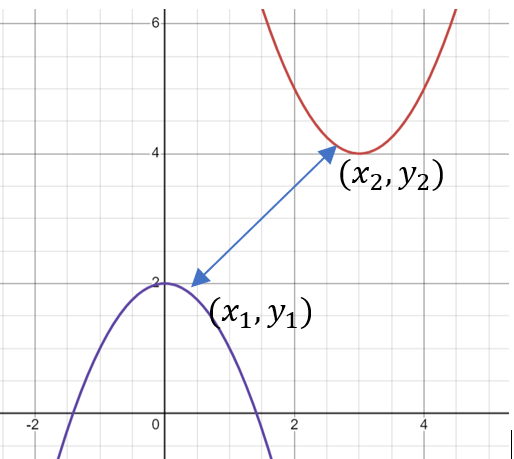
\includegraphics[width=0.25\linewidth]{images/t2w1q2_a.png}
    \end{figure}
    Firstly, we know that at this minimum distance the normal to each curve will have the same gradient, therefore their tangents have the same gradient.\\
    \(y=-x^2+2\)\\
    \(y'=-2x\)\\

    \(y=(x-3)^2+4\)\\
    \(y'=2(x-3)=2x-6\)\\

    These occur at different x values, but we can still equate them by using \(x_1\) and \(x_2\) to represent these points.\\
    \(2x_2 -6=-2x_1\)\\

    Rewriting so that we have one x value in terms of the other:\\
    \(x_2=3-x_1\)\\

    The formula for distance between the curves is:\\
    \(d=\sqrt{(x_2 -x_1)^2+(y_2 - y_1)^2}\)\\

    Which becomes \(d=\sqrt{(3-2x_1)^2 +(y_2 -y_1)^2}\)\\

    We can also find expressions in terms of \(x_1\) for \(y_1\) and \(y_2\):\\
    \(y_1=-(x_1)^2+2\)\\
    \(y_2=(x_2 -3)^2+4=(3-x_1 -3)^2 + 4=x_1^2+4\)\\

    Substituting these into distance:\\
    \(d=\sqrt{(3-2x_1^2)^2+(2x_1^2 + 2)^2}\)\\

    This formula gives the distance between the curves, so we just need to minimise this.\\
    Simplify then differentiate. (Note: I have written \(x_1\) as x from this point on just to simplify the working.)
    
    \(d=\sqrt{9-12x+4x^2+4x^4+8x^2+4}\)\\
    \(d=\sqrt{4^4+12x^2-12x+13}\)\\

    \(d'=\frac{16x^3+24x-12}{2\sqrt{4x^4+12x^3-12x+13}}=\frac{8x^3+12x-6}{\sqrt{4x^4+12x^2-12x+13}}\)\\

    Make it equal to zero and solve to find the minimum:\\
    \(8x^3+12x-6=0\)\\
    \(x=0.442\)\\

    Substituting this into the distance formula, we get:\\
    \(d=\sqrt{4(0.442)^4+12(0.442)^2-12(0.442)+13}=3.193\)\\
    \begin{figure}[H]
        \centering
        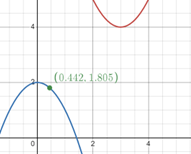
\includegraphics[width=0.25\linewidth]{images/t2w1q2_a2.png}
    \end{figure}
    
    \item 
    Use the change of base formula:\\
    \(y=\frac{\ln{x}}{\ln{a}}=\frac{1}{\ln{a}}\times \ln{x}\)\\

    \(y'=\frac{1}{\ln{a}}\times \frac{1}{x}=\frac{1}{x \ln{a}}\)

\end{enumerate}

\end{document}